\chapter{Experiment}

\par We carried out an experiment at California Polytechnic State University to test the efficacy of habit-based educational software. We created a web-based application called \textit{Polycommit} that was connected to 4 college classes: \textbf{Introduction to Computer Networks}, \textbf{Introduction to Computer Graphics}, \textbf{Introduction to Computer Networks}, \textbf{Introduction to Operating Systems}, and \textbf{Linear Analysis I}. These classes were selected because they covered subject matter that was easy to convert to online quizzes. For instance, one staple Linear Analysis problem is to find the determinant of a matrix (often a whole number), which is easy to input into an online form. In addition, I had taken these classes in recent quarters and was familiar with the course content. 

\par We presented Polycommit to each of the courses in the first 2 weeks of class. Students voluntarily signed up through a website hosted at https://polycommit.com/, where they were able to log in with one click through the main Cal Poly portal. This lets students easily access the website, while also guaranteeing that only Cal Poly students can sign up for the program.

\section{UI Overview}

\subsection{Home Scren}
\par Upon logging in, students click "Enroll" for the classes they wish to participate in. Upon enrolling, the classes are listed under the "Enrolled Classes" section (\textbf{\hyperref[fig:polycommit1]{Figure \ref*{fig:polycommit1}}}). This page also lists the two main "scores" that students earn by answering questions: \textbf{Commitment} and \textbf{Points}.

\par Commitment is a numerical value that represents how many \textit{unique} days a student has answered a question on the website. Students could earn up to 1\% extra credit on their final grade in the class by getting 15 Commitment.

\par Points are earned by answering questions. More points are awarded for correct answers, and bonus points are awarded based on the user's current Commitment. All participants in the experiment were placed in a raffle for \$20 Amazon gift cards. Additional entries into the raffle were awarded by earning more points.

\begin{figure*}[h]
	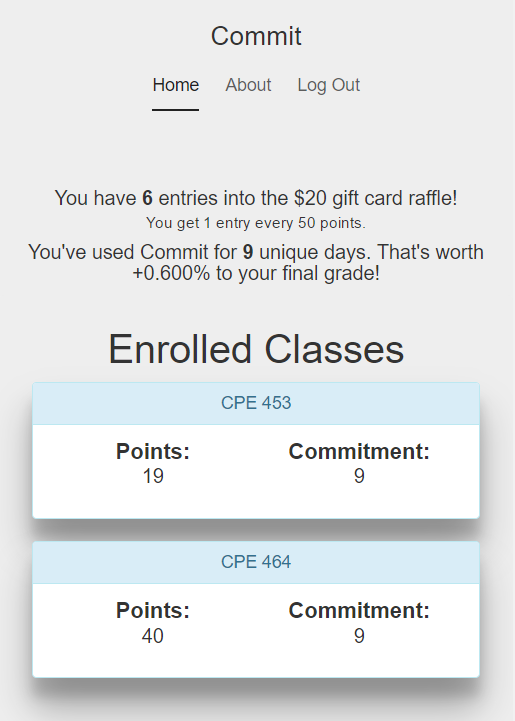
\includegraphics{figures/polycommit-screen}
	\caption{The "Home" screen for Polycommit. Students can see their current progress and can click on a course to answer challenges.}
	\label{fig:polycommit1}
\end{figure*}

\subsection{Course Screen}
\par Each course page has a list of challenges (\textbf{\hyperref[fig:polycommit2]{Figure \ref*{fig:polycommit2}}}) that are open to the student. Challenges are organized into \textbf{Weeks}. If a student has completed all the challenges in a week, the week is displayed with a green check mark and does not expand. If there are open challenges in a week, the week is displayed in yellow with an "alert" icon, indicating that the student has an available challenge. This UI imparts a sense of urgency to the user, since they could potentially lose Commitment by not answering a question each day. Each challenge also lists the date it was opened, and the number of points awarded if the challenge is already completed.

\par Finally, the Course page lists the student's points and Commitment for the course, along with a tooltip that explains what "Commitment" is. This information is repeated from the Home page, since it is the most relevant information for the user, and it is inherently satisfying to watch your points and Commitment rise as you complete challenges.

\begin{figure*}
	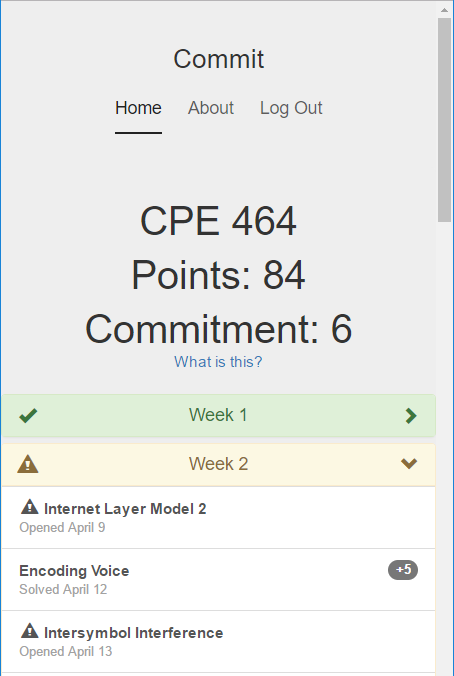
\includegraphics{figures/polycommit-challenges}
	\caption{The "Course" screen for Polycommit. Students can see their current Points and Commitment and can see a list of challenges organized by date.}
	\label{fig:polycommit2}
\end{figure*}

\subsection{Challenge Screen}
\par The challenge screen is where users input 